\chapter{Introduction} 

Organic semiconductors have a niche to fill across the landscape of electronic
device manufacturing due to the flexibility, processability, and cost of manufacturing. 
Organic light emmiting diode(OLED) devices are utilized today in TVs and cellphones.  
Cutting edge foldable OLED screens are commercially available, and a rollable tv was debuted in 2019
\cite{Chen2020}. 
Organic semiconductors are integral to the design of next generation medical devices owing to their
self-healing properties and their biodegradability \cite{Bettinger2010}. 

More generally, the solution processability of these materials allows for
cheaper manufacturing, the consumption of less rare elements, 
and the ability to assemble on curved substrates making for a dizzying array of design possibilities. 
A survey of these materials, and 
other emerging organic electronic technologies, can be found the survey text 
Organic Electronic: Emerging Concepts and Technologies
\cite{FabioCicoiraEditor2013}. 

The materials below are under investigation for their part in the design of organic solar cell (OSC) devices. 
Organic materials used for OSC design are referred to as organic photovoltaics (OPVs) for their capacity
to turn photons into voltage (or voltage into photons in OLEDs). We note that this phenomena is not
local to these molecules, as any molecule is willing to promote an electron to a higher energy level if a
photon of commenserate energy levels is incedent on the molecule. OPV materials are instead distinguished by
their capability for electronic tuning and thier ability to be processed into structures suitable to a specific
design purpose.

OSC devices could afford all the above functional improvements in flexibilty and processability as well as other
potentially revolutionary design capabilites.  
For example, researchers have exploited a unique feature of the physics the excitonic photoabsorbtion in 
organic materials.  Namely, that absorbtion spectrum
in these materials is relatively narrow ($\approx$300nm).
With this, they are able to tune the active layer material to absorb radiation right above or right below the
visible spectrum (into the NIR or UV spectrum respectively). This 
could allow for the production of windows that passively draw current while allowing in natural light. Semi-transparent OSCs have already
reached 11 \% efficeincy \cite{Brabec2020}. 

Two major breakthroughs have ushered us into the modern era of OSCs,
wherein effeciencies are approaching the milestone 20\% effeciency \cite{Liu2020b}.
These are the design of bulk heterojunction (BHJ) active layers and non-fullerene, fused-ring electron
acceptor (FREA) molecules. 

A fundemental physical difference in the nature of photoabsorbtion in inorganic and organic 
semiconducting materials necessitated the
invention of the BHJ. The coloumbic attraction, $V$, between the an excited
electron and the hole it leaves behind in the its molecular orbital
is given by Coulombs law as follows:
\begin{align}
    \label{coulomb}
    V  =  k_{e} \cdot \frac{e^{2}}{\epsilon_{r}}
\end{align}
where $k_{e}$ is Coulomb's constant and $e$ is charge of an electron. Relative permitivitty,
$\epsilon_{r}$, is a unitless quantity that describes a materials polarizability relative
to that of free space. That is, relative
permativity describes the readiness of a material
to polarize in response to an electric field. A
relative permitivitty of $~3$ in OPVs means that these materials are only $3$ times more polarizable than free space, which
is not all that polariazable. And, because the material occupying the space between electron and hole
is not willing (or able?) to fight back against the electric field created between them, they stick together and behave as a quasipartcle. 
This bound electron-hole quasiparticle is refered to herein as an exciton.

[Silicon has a relative permitivitty of ~12. not sure in need this i think its kinda understood]

% keep attachced to prior paragraph
This excitonic absorbtion introduces a unique design challenge.
That is, to extract a charge from the device, the exciton
must first be coerced apart. This coercion can take place at the interface between donor and acceptor molecules,
where the slight offset in energy levels creates a charge transfer state wherein it is more
energetically favorable for the donor to undergo electron transfer with an adjacent acceptor than
it is to radiatively decay to its ground state and photoemit.
This means that, after photoabsorbtion, the exciton must to diffuse to this interface for the charge to be
extracted. An exciton can diffuse roughly 10nm before relaxing \cite{clarke2010}. 
Producing a layer this small is untenable and further a thicker layer
is diserable to interact with as much of the ambeint radiation as possible so as to ``catch'' as many photons
as possbible. 

In 1986, Ching W. Tang
showed that, processed under the right conditions, a blend of donor and acceptor molecules can self-assemble
into what is termed Bulk Heterojunction (BHJ) microstructure \cite{Tang1986c}. 
The interlocking phases of donor accepter molecules, ensure
that an exciton will intersect with the boundary between accepter and donor domains, while also ensuring that
there
is a continuous escape route, albeit labyrinthine, for the free charges to travel on their way to their respective
electrodes. 

\begin{figure}
    \center
    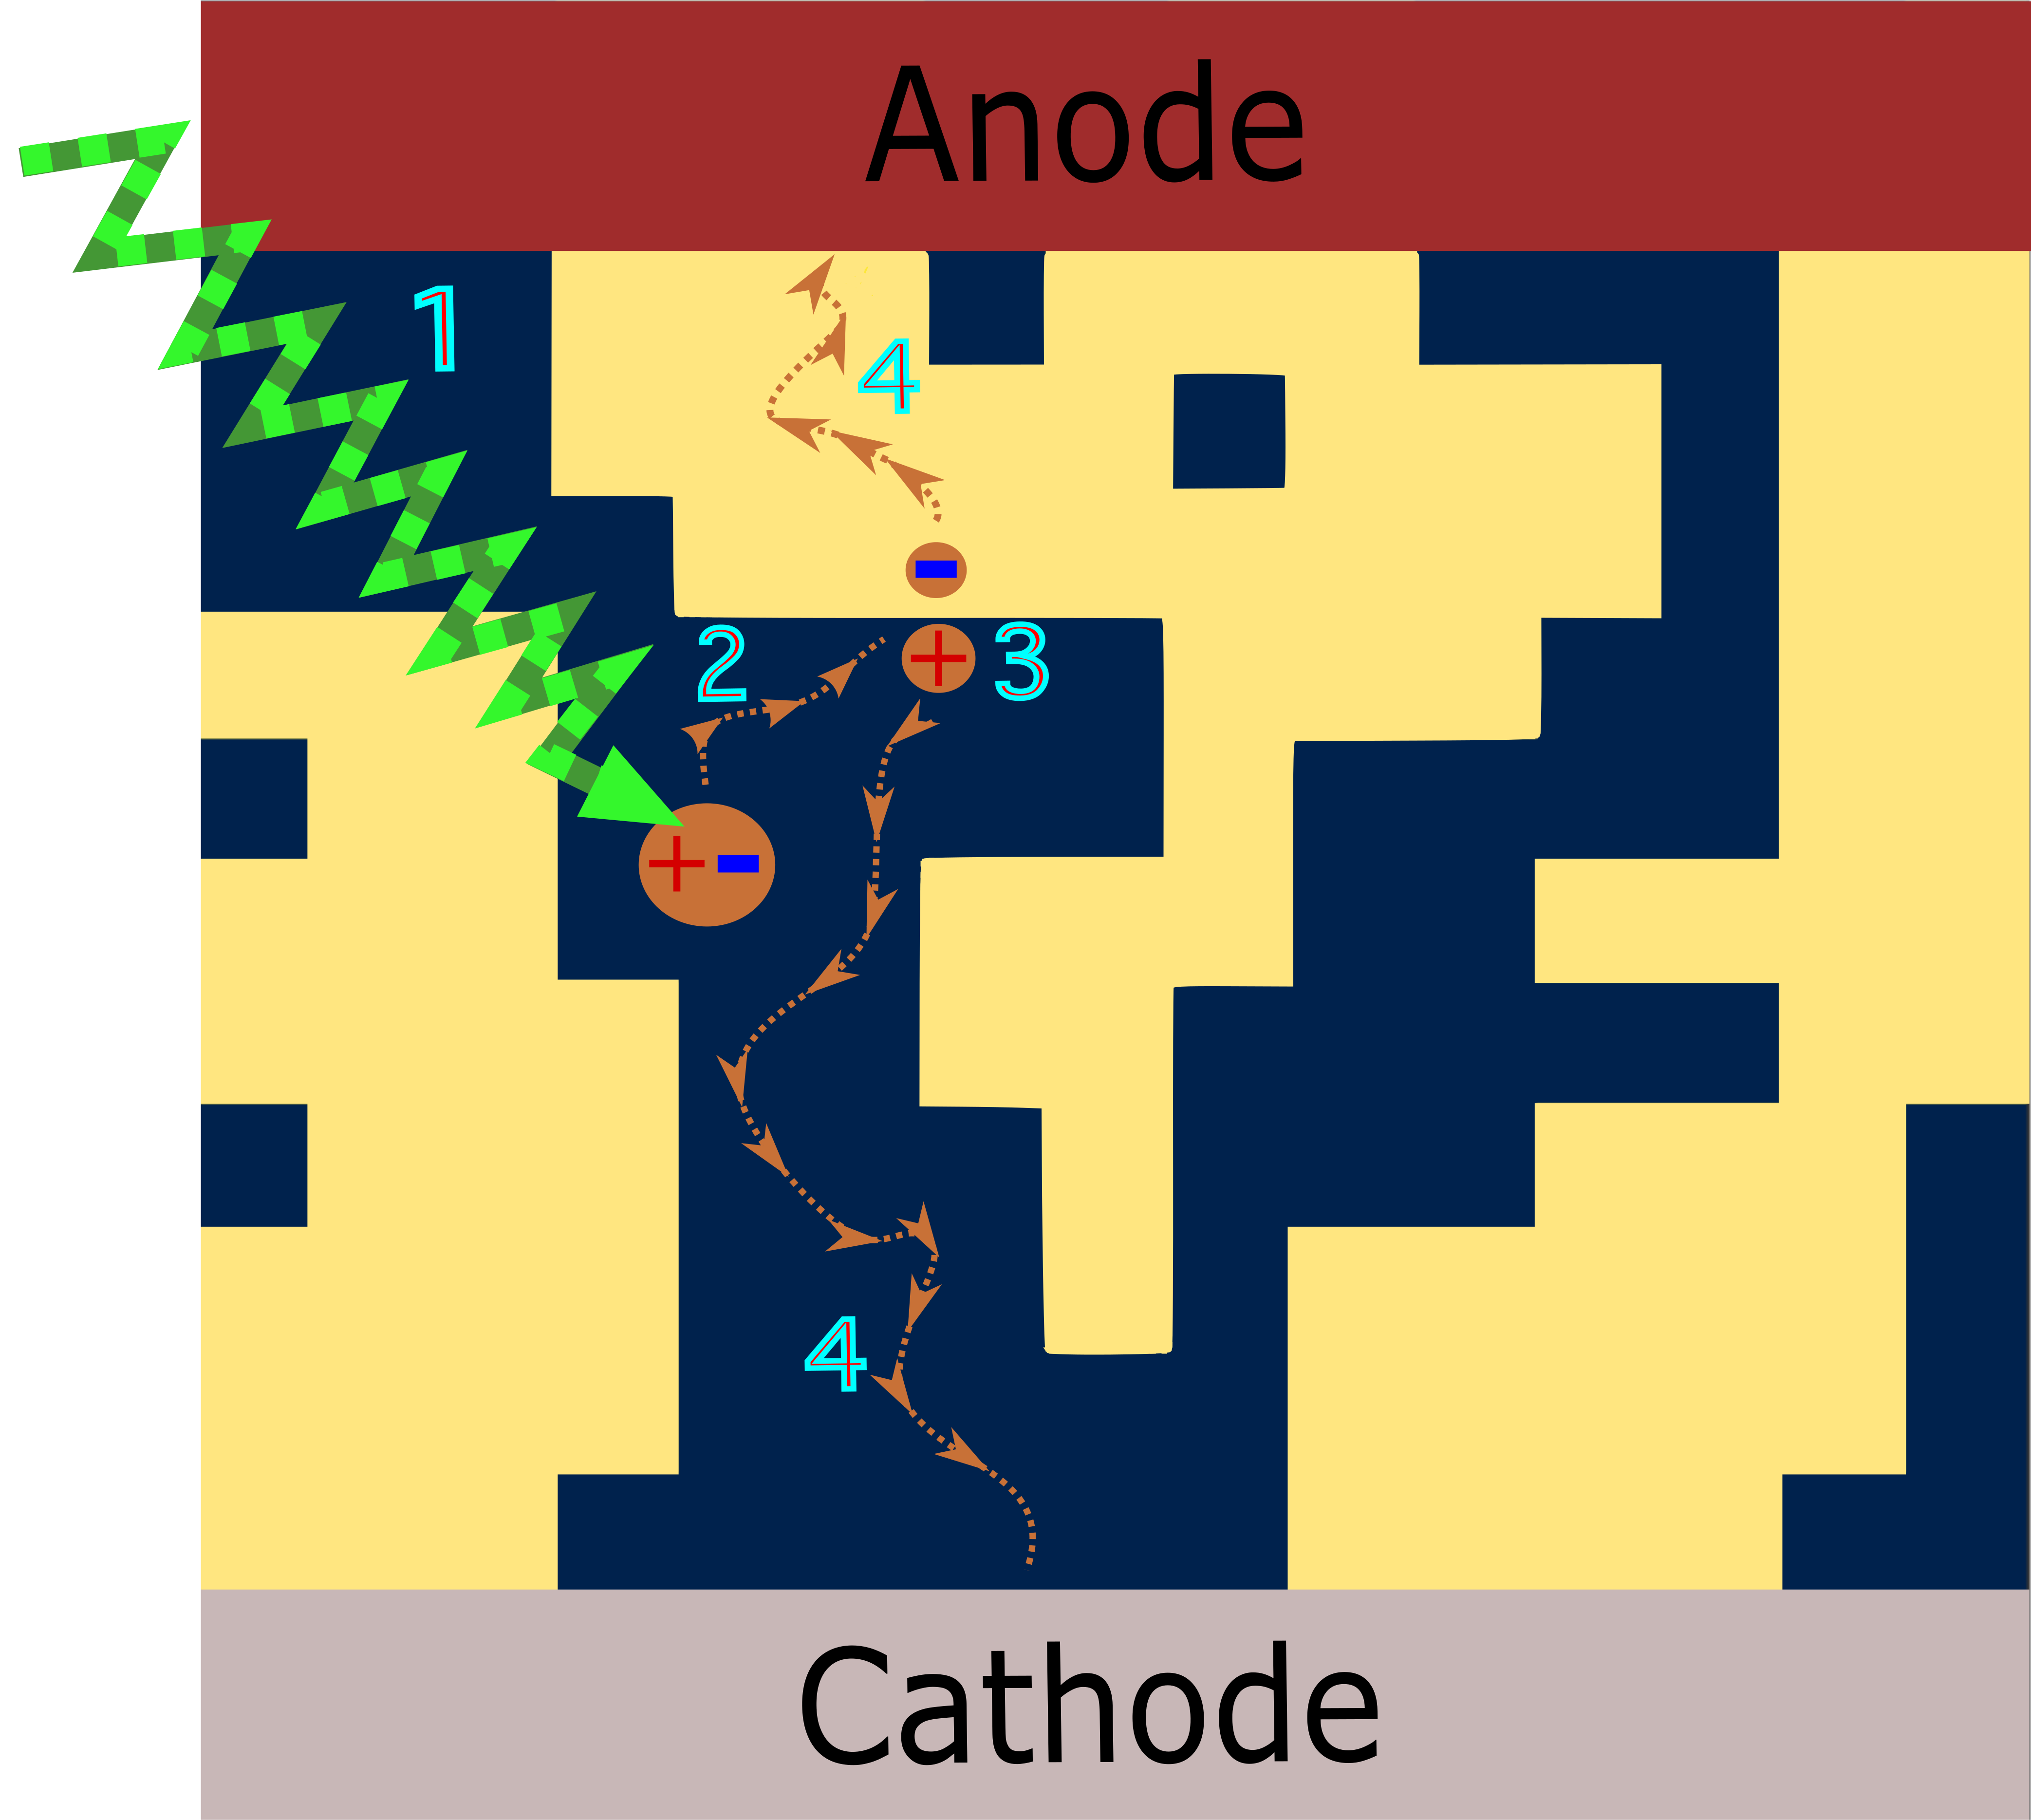
\includegraphics[width = .9\textwidth]{figures/BHJ-figure.png}
    \caption{A cartoon representation of a bulk heterojunction device. All four stages involved in harvesting
    photonic energy in a BHJ device are represtented. (1) The photon (green arrow) interacts with the material,
    exciting an electron and creating an quasiparticle referred to as an exciton. (2) The exciton diffuses
    about until it intersectects the interface between donor and acceptor material domains. (3) The exciton is
    coerced apart by the energy offset between donor and acceptor molecules. 
    (4) The, now unbound,  hole and the electron are free to diffuse about until ther reach their respective
    electrodes where they can be extracted \cite{Fusella2019}}
    \label{bhj}
\end{figure}

% Keep attached to prior paragraph.

As shown in \ref{bhj}, a BHJ active layer is designed to harvest photons through the following 
steps: (1) photoabsorbtions, 
(2) exciton diffusion, (3) charge transfer, and (4) free charge diffusion \cite{Fusella2019}. 
When a photon is incedent on
an OSC active layer, if it intersects with a molecular segment in the donor whose 
highest occupied molecular orbital (HOMO) has comprable energy levels to the photon, 
the energy can be absorbed via the promotion of
an electron to the next available energy level; the lowest unoccupied molecular orbital (LUMO).
This forms an exciton as
described above, which can then diffuse until it intersects the boundary. 
The excited electron would like to relax
back into is lower energy level, but at the interface with the acceptor, it finds a better option. The
acceptor's LUMO is engineered to sit between the energy of the donor's excited electron's energy level and the
available lower energy level. Because of this, the electron cascades down to the acceptors LUMO through a charge
tranfer reaction. Finally the free charges can diffuse until they interect the electrode where it can be
extracted. This is, of course, an ideal description, as there are loss mechanisms at all four stages. 

% CURRENTLY Says: Too many things: Active layer structure good and bad, our work focuses on pure domains, space-charge buildup is a thing. 
% SHOULD Say: Something more about solution processability and how it dictates structure, focus in on the structure of the pure domains, and pull out space-charge buildup for its own paragraph (or move in CT mechanisms above)
Our work in this work
is most expressely related to stage four in that we seek to simulate the self-assembly of pure acceptor or
pure donor domains post deposition and simulate free charges moving
through the resulting morphology. These materials can be deposited from solution.
How these materials will self-assemble in the environment in which they are deposited determines
the morphology.  Successfully doing so could inform the ideal conditions for optimizing the morphology.


The charge mobility of both donor and accpetor
are known to be relevant to overall device performace \cite{Wang2019e}.
An understanding of why this is the case can be found from the inspection of \autoref{bhj}.
If the electrons in stage 4 reach the andode much faster than the holes reach the cathode, a traffic jam can
occur at the anode which causes losses. 
Further, imbalanced charge-carrier mobility of this kind can lead to space-charge build up in the 
low mobilty material that can screen the built in field \cite{Bartelt2015}.
This phenomena has been shown by space charge limited current experiments \cite{Small2013}.

% CURRENTLY Says: A bit about the history of PCE, but also here's our first mention of DFT for some reason.
% SHOULD Say: History of PCE. But where does it fit? After paragraphs talking about optimizing structure and optimizing chemistry? 
The BHJ design pushed the effenciency beyond the 1\% effeiciency milestone. Early BHJ devices utilized
fullerene derivitives as acceptors. In 2015, a group of researchers conceptulized the use of
fused-ring electron acceptors, a class of non-fullerene acceptors. This class of molecules consists of
a fused-ring core and end groups that can be engineered to acheive specific electronic characterstics and side
chains that can be engineered to achieve desried morphological features. The modularity of FREAs
layed the stage for headspinning progress in the following years from 4\% PCE to 18\% \cite{Wang2021a}. 
This designed modularity is a benifit to reseachers, as they can alter one component of the molecule and test
the effect on resulting charge charactoristics. For example, in a paper published in 2019 \cite{Benatto2019},
researchers, knowing that flourine is an electronegative atom, swapped 4 hydrogen atoms for flourine atoms on
the end groups of the ITIC molecule. Using density functional theory(DFT), they found 
that this substitution could lower the exciton
binding energy (discussed above using \autoref{coulomb}), thus facilitating exciton dissasociation (stage 3 of
BHJ). They also found
that this flourination tends to reduce the reorganization energy, which we see in \autoref{results}, has a
drastic effect on charge mobility.

% CURRENTLY Says: Trial and error is hard, DFT is hard, and software is closed. Too much! 
% SHOULD Say: We're at least missing a paragraph that says something about how simulations can help us choose which things to make in real life, and perhaps a summary of some of the techniques, what they are, and how they differ. That'll set us up for talking about MD in one paragraph and DFT in another paragraph, their strengths, and hint or preview at how we might use them in this work.
This type of molecular tinkering is a critical first step that can lay the groundwork for further wetlab
experiments and can ultimately inform device design. Unfortunately, the molecular modularity of FREAs is not
mirrored in the software used to study them. DFT is prohibitivly slow on the nanometer
scale. Furthermore, investigations like these rarely publish the code necessary to reproduce or extend the
work, and often utilize proprietary software. On the contrary, the software used in this 
work is maintained in public. In the
case of MorphCT, actively developed for this thesis, workflows are
also maintained in public. These workflows, maintained as jupyter notebook tutorials, 
are meant to lower the cognitive load of taking on a research project in this vein. 


% CURRENTLY Says: Summary of what we focus on, but also definitions of terms.
% SHOULD Say: Something about acceptors and donors, which means it should go after a description of acceptor and donor moieties, and maybe after a description of structure
In our present work, we present results from a computational investigation of two OPV materials
used in the design of the active layer of organic solar cells (OSCs). These are P3HT, a
donor molecule, and ITIC, an acceptor molecule. With respect to organic electronic devices, `acceptors' are the
organic analogue of p-type inorganic semiconductors and `donors' the analogue
of the n-type. We make this note because in the methods we describe a model of
a charge `hopping' from one molecule to another. And as we describe, our
investigation involves hops within a pure donor domain or within a pure
acceptor domain. A common point of confusion is distinguishing between which
molecules are donors or acceptors.
Any molecule can accept or donate a charge carrier OPV.
They merely receive their donor/acceptor designation as a result of how they
are primarily utilized in electronic devices. 

% CURRENTLY Says: Definitions of P3HT and ITIC
% SHOULD Say: Maybe a bit more about these molecules, but this needs to go after a generic description of OSC's (why OSC and not OPV that we use everywhere else?). 
P3HT is a polymeric material that is highly polymorphic in that it can self-assemble into a wide spectrum of
crystallinities depending on how it is processed. Shown in \autoref{molecules}, the molecular struture of P3HT
is such that these molecules can pi-stack into lamalear strucutes. 
P3HT was first synthesized by Rick Mcullough in 1992. Polythiophenes as a whole have been well investigated 
since 1883 when they were first characterized.\cite{Poelking2014}.
ITIC is not polymeric. Rather, it a material consisting of small molecules and thus has no long range bonding.
It was first synthesized in 2015 \cite{Bai201U}

\begin{figure}[]
\centering
\begin{subfigure}{\textwidth}
    \centering
    \textbf{(A)} P3HT \\
    \includegraphics[width=.9\textwidth]{figures/p3ht-molecule-figure.png}
    \newline
\end{subfigure}%
\\
\begin{subfigure}{.5\textwidth}
    \textbf{(B)} ITIC
    \centering
    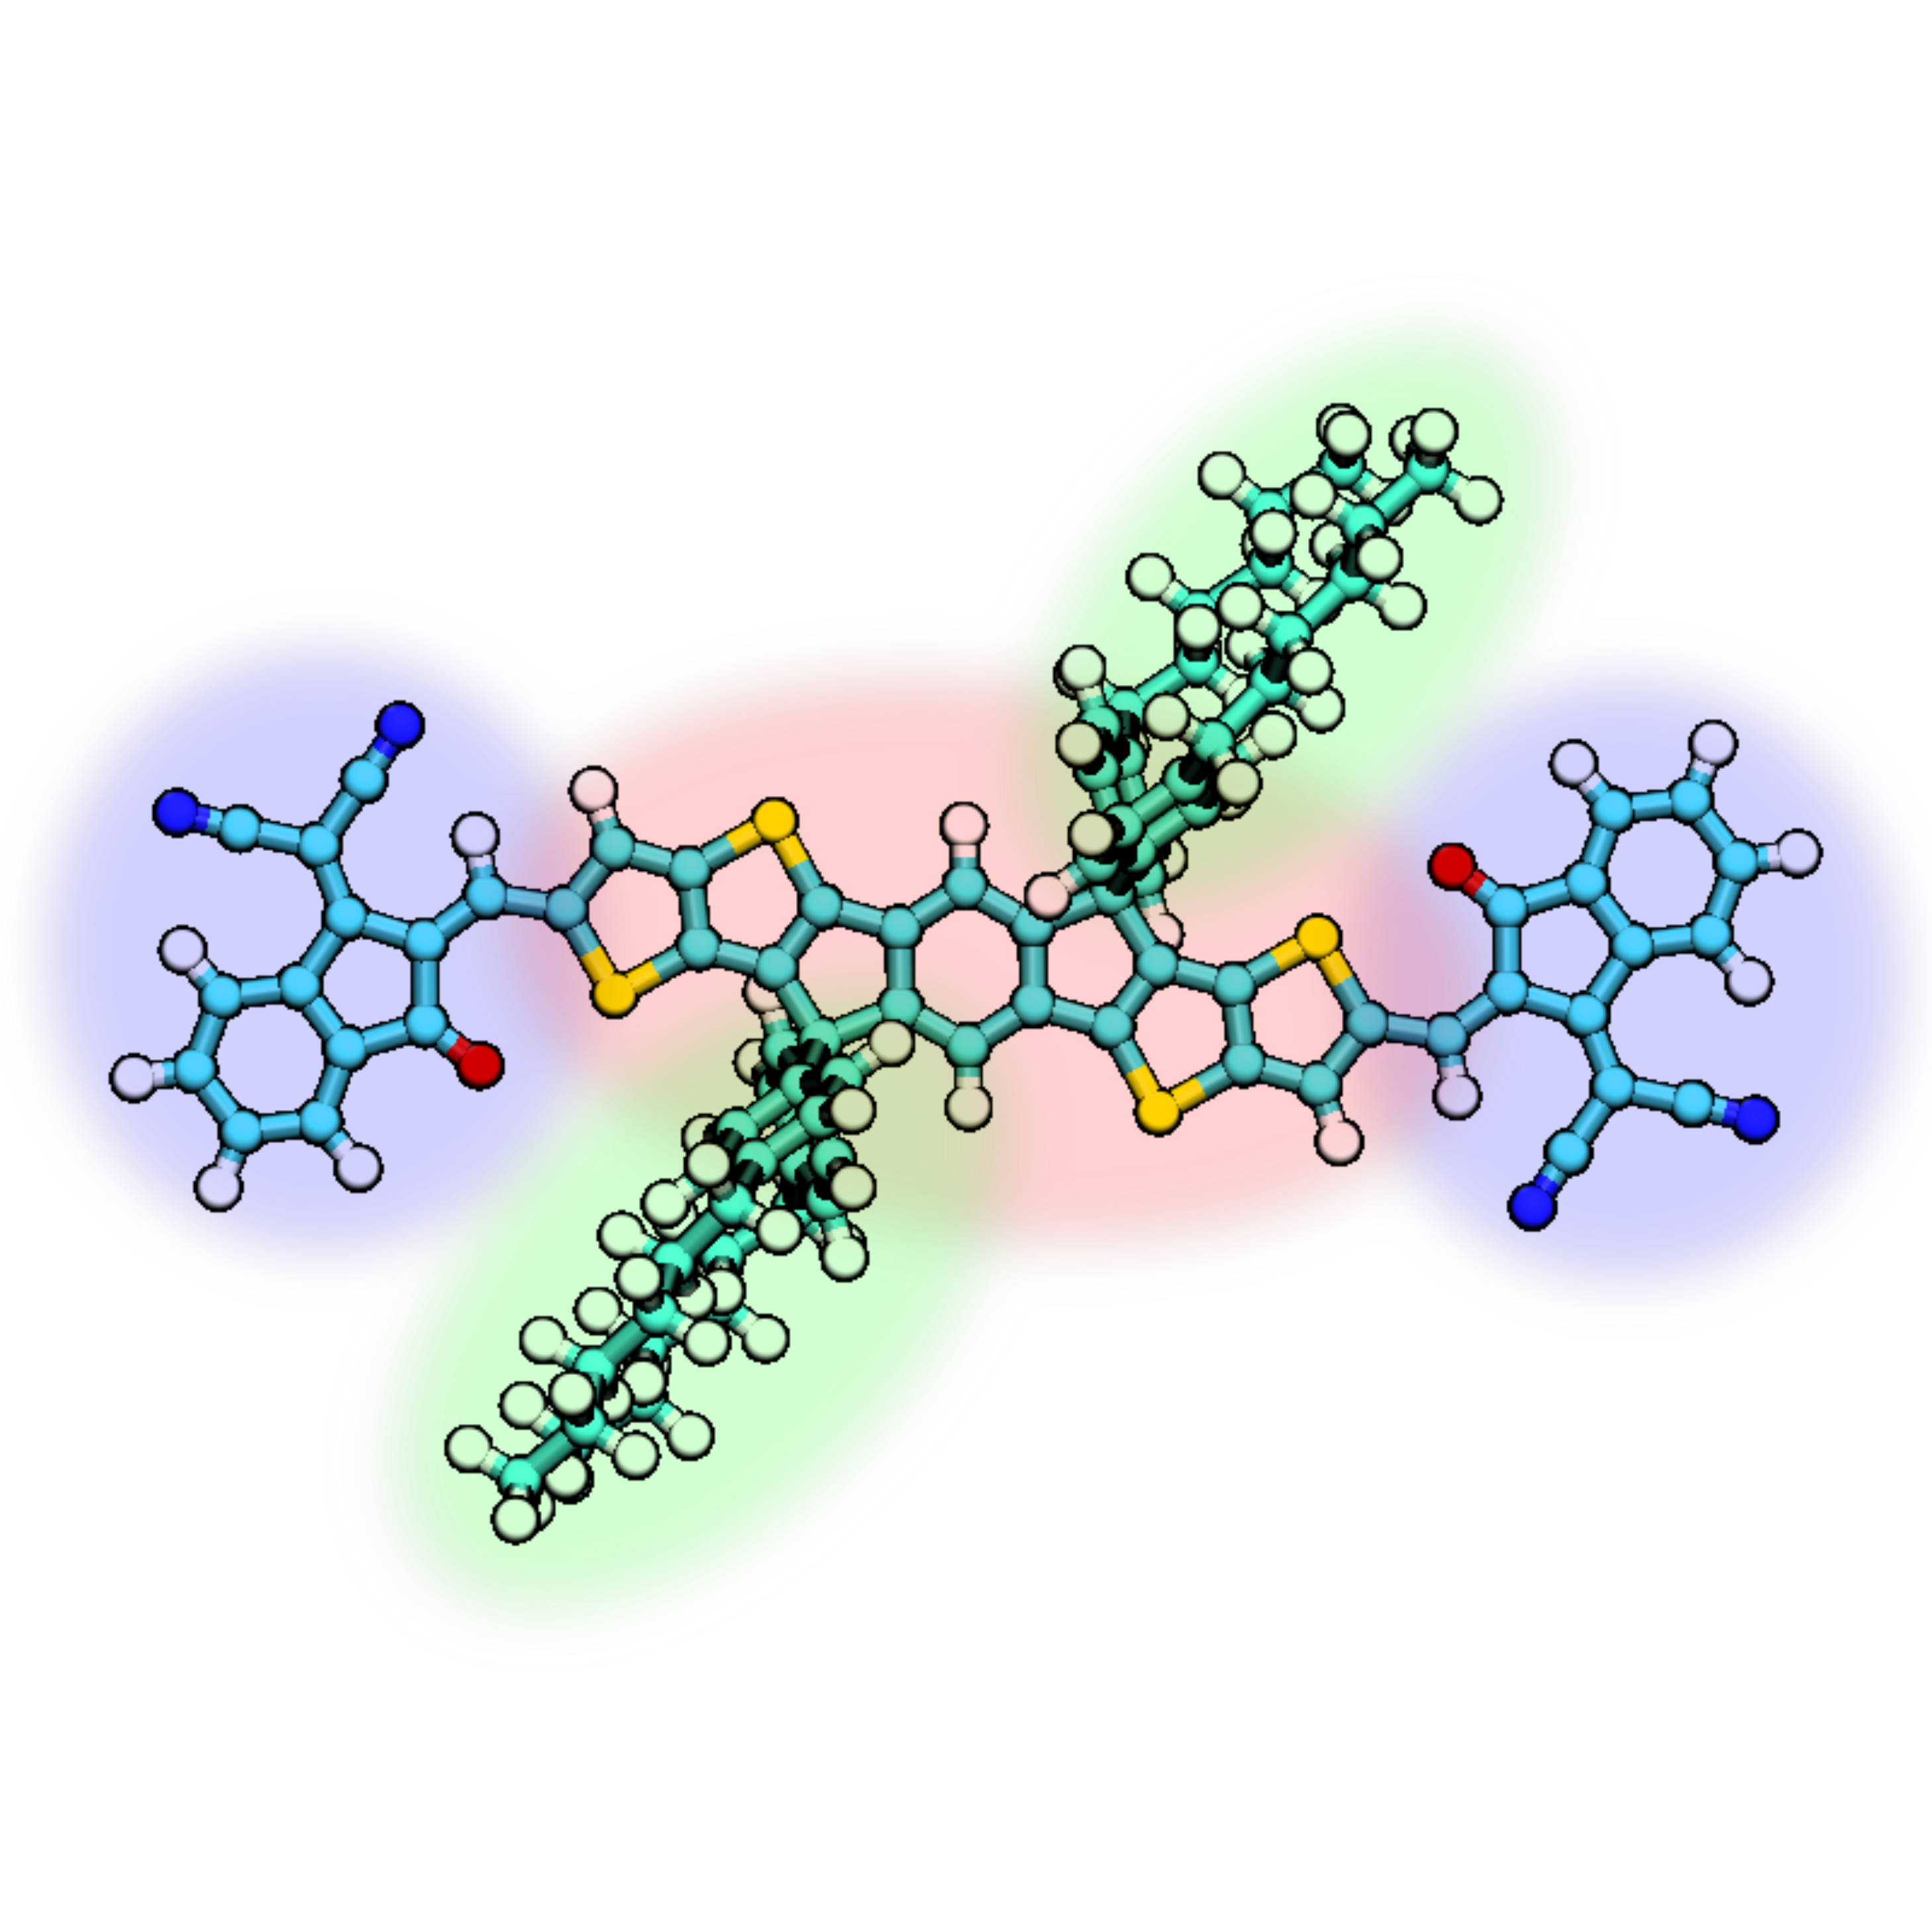
\includegraphics[width=\textwidth]{figures/itic-backbone-figure.png}
\end{subfigure}%
\begin{subfigure}{.5\textwidth}
    \textbf{(C)} ITIC
    \centering
    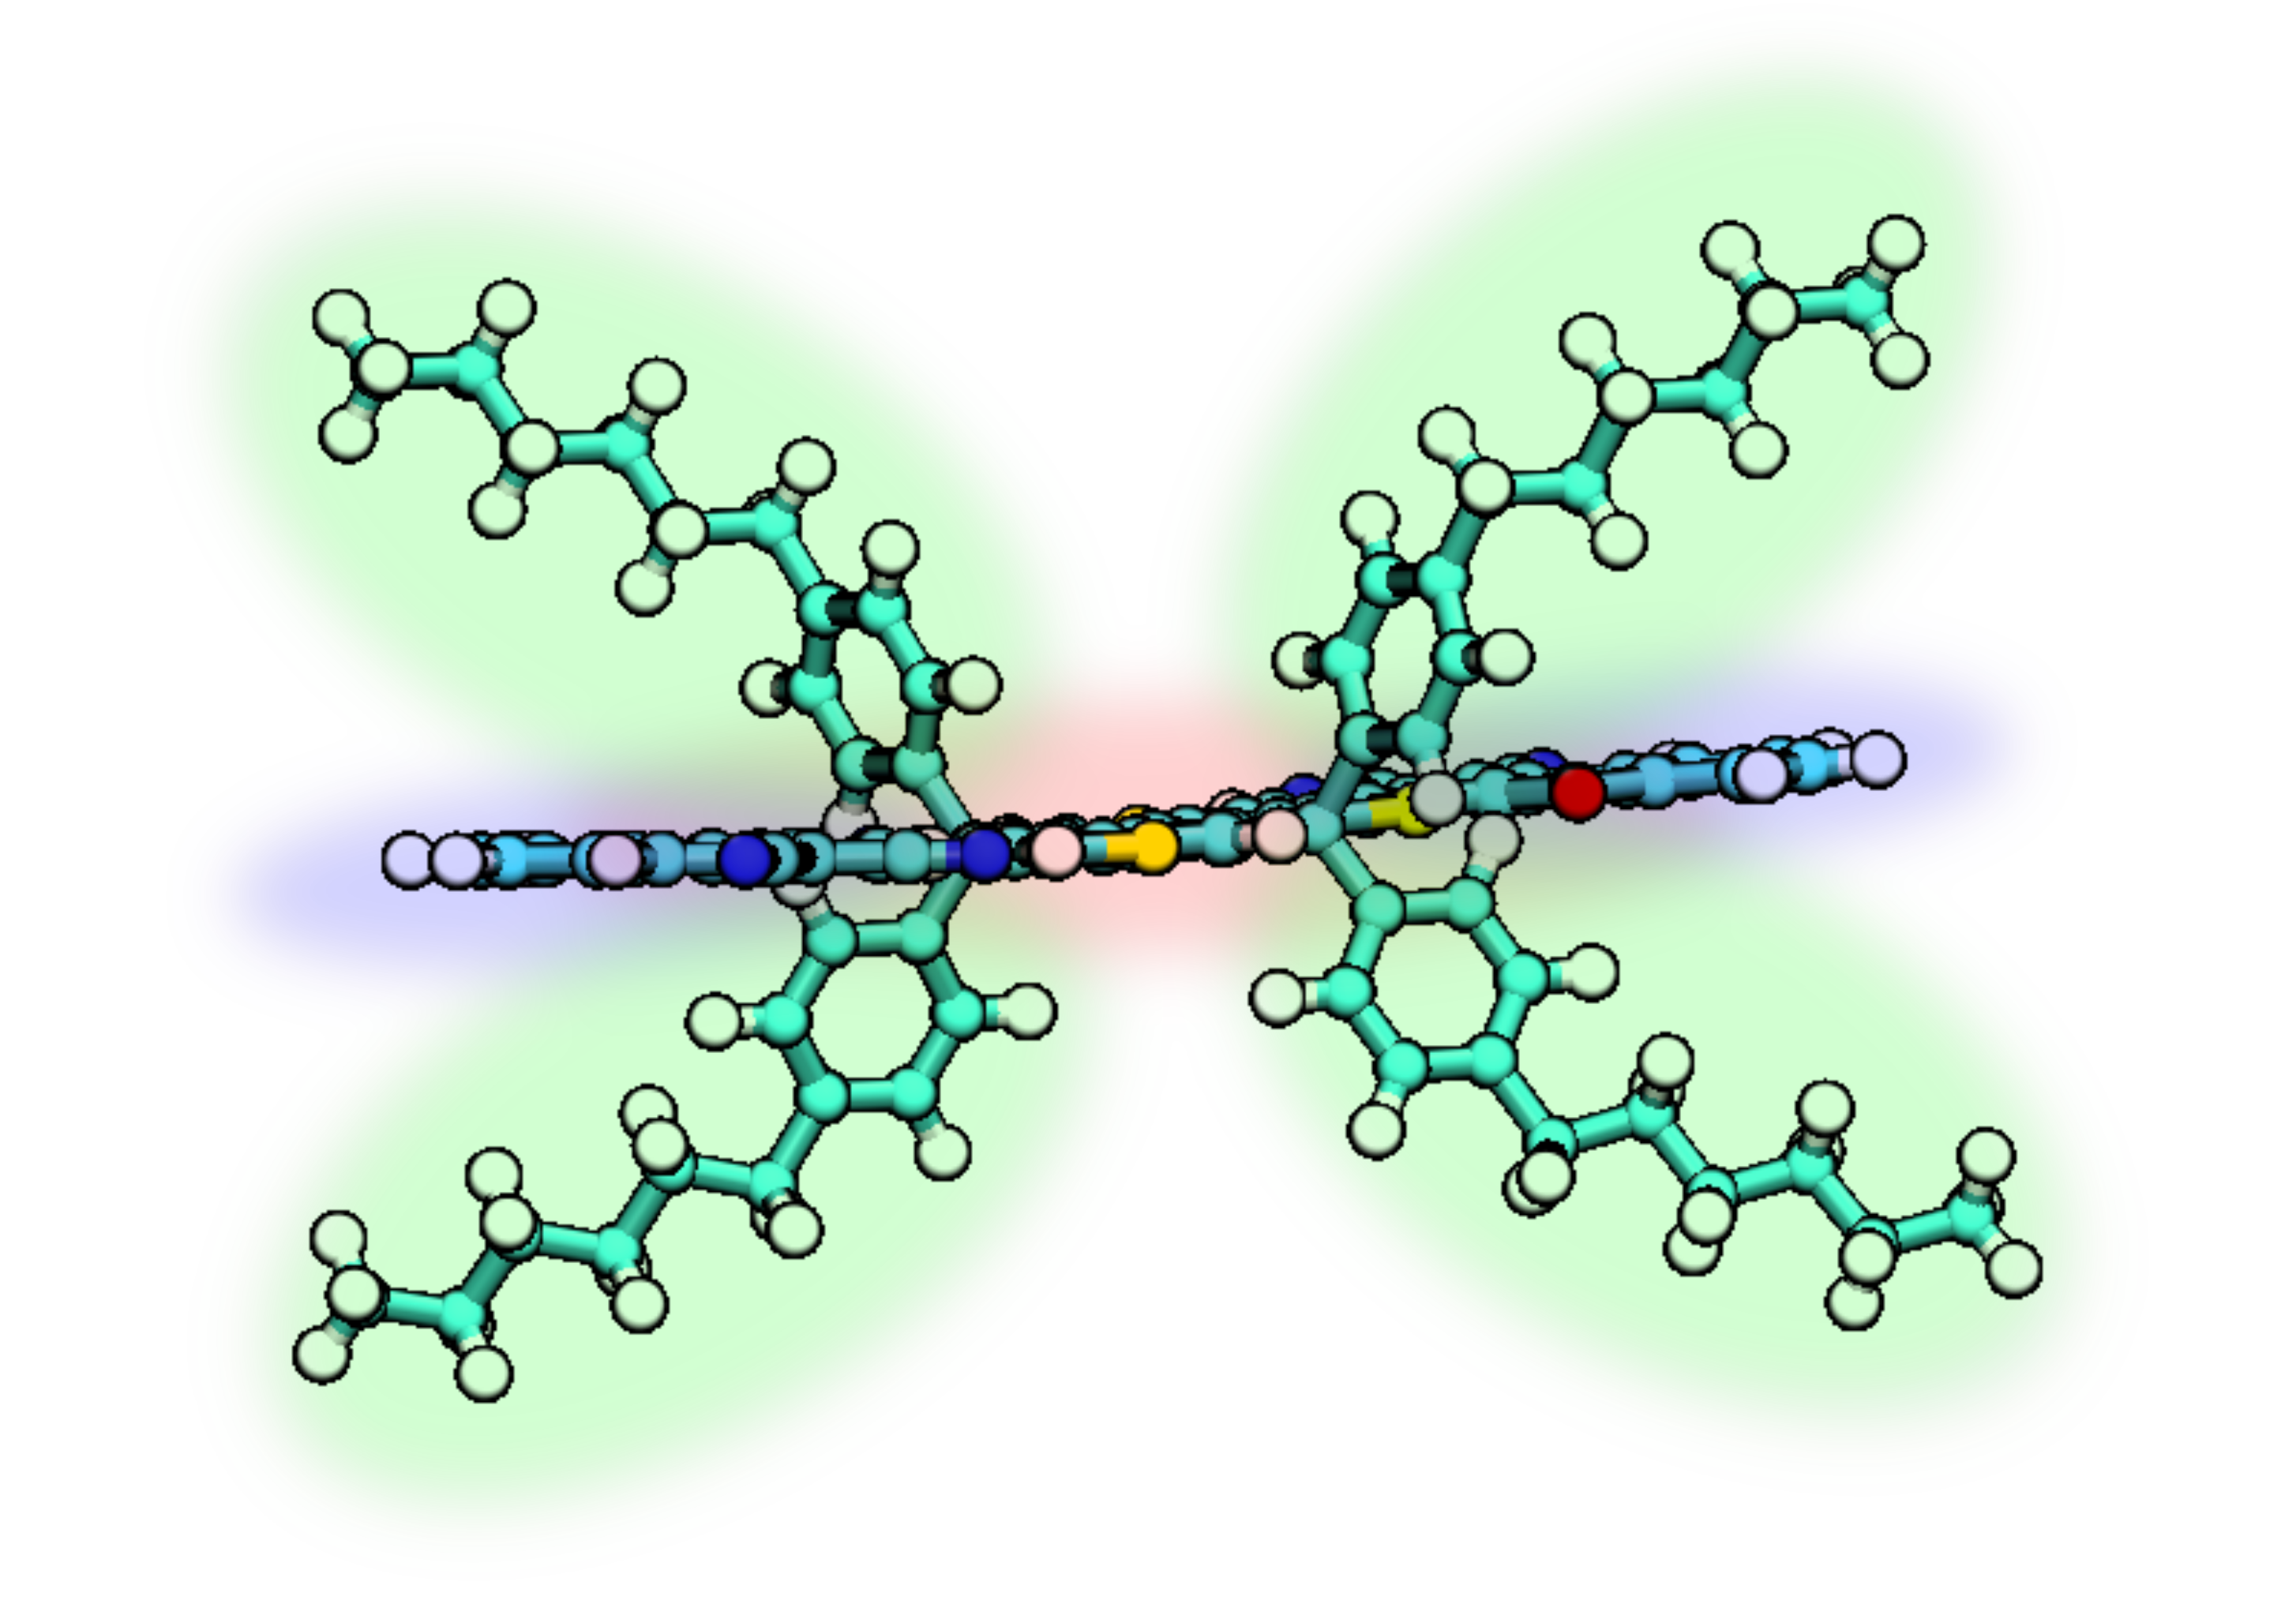
\includegraphics[width=\textwidth]{figures/itic-sidechain-figure.png}
\end{subfigure}
    \caption[short]{(A) P3HT oligomer composed of 15 identical monomers imbued in blue.
    (B) ITIC molecule viewed from above the plane of the backbone. 
    (C) ITIC viewed in the plane of the backone to show the side chains. ITIC
    molecule is imbued with blue, red, and green to call attention to the end groups, fused-ring core, and
    side chains respectively.}
\label{molecules}
\end{figure}

% CURRENTLY Says: We need a modular pipeline to do this sequence of things.
% SHOULD Say: The sequence of steps for going from chemistry to charge transport. Wait till another paragraph for modularity. This will be a good place for a figure of ``the pipeline''
Taking for granted that electronic devices utilizing OPVs is an exciting
space, and with the immensity of the parameter space involved in molecular design, it is desirable that a modular
open-source pipeline exhist for simulating the morphology of candidate molecules as well as simulating the 
associated charge charecteristics. Jones2017 has laid out this
pipeline in detail. To begin, equillibrium molecular dynamics (MD) simulations can predict the chemical
structure of OPVs. The data obtained from these simulations can then be fed as an input into kinetic monte
carlo (KMC) simulations that characterize charge mobility (conductivity) in these chemistries. We introduce MD
and our software stack used to implement it in \autoref{results}. The focus of this thesis, however, involves
the second leg of the pipeline; KMC simulation methods and software are explore in detail in autoref{results}.
\begin{figure}
  \center
  \includegraphics[width=0.99\linewidth]{figures/pipeline-figure.png} 
    \caption{The pipeline used to go from blah to blah}
  \label{pipeline}
\end{figure}

% SHOULD Say: What a chromophore is. talk about chromophores, charge delocalization, and hopping in the context of structure and OPVs here is good.
Stage 4 of the BHJ, the movement of charges through pure domains can be modeled as a particle hopping 
to and from nearby frontier molecular orbitals.
The generic hopping model goes as follows: the wave functions of
free charges are localized on particular molecular segments due to the lack of long range electronic strcuture
, and the movements of these charges can be described as series
of hops bewtween these molecular segments. Where, and to what extent, charges delocalize can been investigated
[REFS]. 

In the \autoref{results} we explore the delineation of these delocaliztion segments, which we hereafter refer to as a
``chromophore.'' 
The term chromophore arose in a biochemical context and is generally defined
as a light-absorbing group or molecule \cite{biochemistry}.
In this context, a chromophore is often associated with the color of a material.
This is because, mechanistically, a photon collides with a chromophore, the absorbed energy
excites an electron from the HOMO to the
LUMO. When the chromophore relaxes to its
ground state, it releases a photon with wave length (or color) $\lambda = \frac{\hbar c}{E}$,
where $\hbar$ is Plank's constant, $c$ is the speed of light, and $E$ represents the
energy difference of the HOMO and LUMO. In plants, this amounts to a rejection of the overabundant amount of
light in the green region which can damage the plant's DNA. 

% CURRENTLY Says: More chromophore details, but also something about photon release
% SHOULD Say: About the same stuff, but this should tie into the structure, sequence of charge generation discussion above.
Our BHJ active layer amounts to a kind of synthetic photosynthesis (woof), and with that we have no DNA to
protect and no colors emitting from our devices. We nevertheless continue with the use of the term chromophore
for the sake of brevity. In what is to follow, chromophore is taken to be defined as a molecular segment over which the 
wave function of an electron (hole) is thought to be fully delocolized in a pure accpetor (donor) domain. 
It is under this assumption that we execute a hopping model of charge transfer between
chromophores based on the Marcus rates of electrochemical reactions.  

% SHOULD Say: More about what TRUE is, why we think it's good, and then pivot to talking about how modularity is can help with TRUE. 
TRUE materials simulation tools are developed with an emphasis on creating tools that are
transferable, reproducable, usable, and extensible (\cite{Cummings2017}).
With scientific research being an innately distributed endeavor, these virtues provide a lens through which to
evaluate the adherence to basic scientific principles and to the best practices of distributed software development
simultaneously. As enumerated by Jankowski et al, some of emerging best practices for scientific software
development include the following: (1) address cognitive load, (2) use version control, (3) automate
repetitive tasks, (4) develop open-source code, (5) write code in the highest language possible
\cite{Jankowski2020}.


% SHOULD Say: Thesis summary. Add a sentence or two on each of (a) your thesis plan, (b) what you found, (c) what it means. 
In this thesis, we seek to improve the TRUEness of the pipeline outlined above, with particular attention
to the charge characterization.
Our goal in this work was to: (1) integrate the fully open-source QCC software pySCF into MorphCT,
(2) test the new pipeline/software stack (3) develop facilitatory workflow materials for navigating the
pipeline across the kaleidoscope of scientific theory and software packages. 
We found that the pipeline can indeed connect moluclar sturcture to morphology to charge
mobility. As with other software the greatest hitch to the TRUEness is the
cognitive load. The cognitive load I found most overbearing was the quantum theory underlying the algorithm 
at the molecular level and the cognitive load of learning the MorphCT API. 
I also found that the most useful tool to onboarding the MorphCT API was the
trail of breadcrumbs left by previous developers on github issues, documention and tutorials. 
With that workflows codified into jupyter notebook tutorials are the resourse that I would want if I was to
attempt this research again and therefore are my best attempt to bring an aspiring developer into the fold.
We have found that interactive tutorials provide an exposure to the MorphCT while also shoring up the
theoritcal gaps in knowlegde necessary to navigate this kind of research. 

In \autoref{methods}, we
give an exposition of the theories and software packages used to model and simulate self-assembly and charge mobility in
OPVs.
The methods used in this thesis are centrally motivated by, and justified for, 
the application of our workflow to materials
used in OSC desing. However, the methods are
not exclusively applicable to these materials and could be applied similarly to supplement the engineering of any organic
electronic devices, like those mentioned above. 
Version one of MorphCT was capable of
connecting qualitativley the morphological features produced by MD simulations. However, it was determined
that in the interest of reprducabitilty, it was critical to ``containerize'' this pipeline. Until as recently as
the past few years it was common place to not publish code with the results of computational works. Containers
are virtual machines that contain all the dependencies, configurations, code and data necessary to reproduce
results. \cite{Cito2016a}


% CURRENTLY Says: Results summary.
% SHOULD Say: Same, but smoosh into above paragraph.
In \autoref{results}, we use MorphCT to validate our current workflow against a predecessor of the 
workflow on three benchmark MD simulated morpholgies of P3HT. 
Following that, again using P3HT, we test the sensitivity of our KMC algorithm, implemented
implemented with MorphCT, to a variety of inputs. We conclude \autoref{results} by applying our pipeline,
start to finish, to ITIC. 

In \autoref{conclusion}, we outline the ramification of \autoref{results} and detail the areas of future
development of the workflow. 

THIS SENTECE HAS NO HOME Researchers have to
balance the optimiztion of electron structures of candidate donor/acceptor materials against the miscibility
of two candidate molecules as well as the resultant morphology across the thermodynamic landscape of
variuos solution processes which ultimately govern the Jsc and FF of at the device level \cite{Zhu2020a}. 
%%% Local Variables: 
%%% mode: latex
%%% TeX-master: "BSUmain"
%%:set textwidth=80
% End: 
